\documentclass[twoside]{article}
\usepackage{ecj,palatino,epsfig,latexsym}
\usepackage{url}
\linespread{1.6}
\usepackage{graphicx}
\graphicspath{ {images/} }
\usepackage{amsthm,amsmath}
\usepackage{framed}
\usepackage[utf8]{inputenc}

%% do not add any other page- or text-size instruction here

\parskip=0.00in



\begin{document}

\ecjHeader{}{}{}{}{Caribou and Canis Lupus in North America}{Alverson and Trifunovski}
\title{\bf Effect of climate change on the distribution of Caribou and Canis Lupus in North America}

\author{\name{\bf Maximilian Alverson} \hfill \addr{malverson@wesleyan.edu}\\
        \addr{Biology Major, Wesleyan University,
        Middletown, 06459, CT, USA}
\AND
       \name{\bf Maksim Trifunovski} \hfill \addr{mtrifunovski@wesleyan.edu}\\
        \addr{Computer Science, Wesleyan University,
        Middletown, 06459, CT, USA}
}

\maketitle

\begin{framed}
\begin{abstract}

  \section*{Background}
  Caribou refers to the North American subspecies of Rangifer tarandus,
  also known as the Reindeer in Europe and Asia. North American populations
  of caribou primarily inhabit the tundra and boreal forest ecosystems,
  presently ranging from Alaska across most of northern Canada. The gray
  wolf (Canis Lupus) is the primary predator of caribou, and is found in
  much of the same habitat as the caribou. On the other hand, caribou's
  main food, especially during winter when other food sources are not available,
   is fruticose deer lichen (Cladonia rangiferina), and it is also
  found in much of the same habitat. Because arctic environments and
  the species inhabiting them are particularly vulnerable to the effects of
  climate change, the natural distributions of the caribou, the gray
  wolf and the reindeer lichen are expected to change in the near future
  due to the adverse effects of climate change. To analyze the effect of
  climate change, climate data variables such as temperature and precipitation,
  are measured at present time and by using climate models to predict the
  conditions in 2070.

  \section*{Results} %if any
  Using maximum entropy (Maxent) species distribution modeling, we examine
  the current distribution of Rangifer tarandus, Canis Lupus and Cladonia
  rangiferina on the continent of North America, predict the possible
  distribution in 2070, and attempt to explain the various factors that
  influence the distribution of caribou, gray wolves and reindeer lichen.
  The results show us that the suitable habitat area of the Caribou shrinks
  by quite a lot, while the habitat of the gray wolves and the lichen remain
  almost the same.

  \section*{Conclusions}
  The main conclusion that we can make is that the distribution of caribou will
  shrink due to the effects of climate change, even though food sources such as
  Cladonia Rangiferina will still be available. While the results of the
  habitat change of gray wolf are inconclusive, we have to consider what the
  lesser numbers of Caribou, the gray wolf's main food, will mean for
  the distribution of gray wolves in North America. However, it is important to
  note that the analysis of these species' distributions only took into account
  the effects of climate change based on climatic variables. Other anthropogenic
  factors such as increased human activity in the arctic and tundra regions are
  also likely to have an impact on many arctic species, including caribou and
  grey wolves.

\end{abstract}

\begin{keywords}

Caribou,
Raindeer,
Canis Lupus,
Gray Wolf,
Reindeer lichen,
Cladonia rangiferina,
Maxent,
Climate change.

\end{keywords}

\end{framed}

\section{Introduction}
Our research involved three species: Reindeer lichen (Cladonia rangiferina),
caribou (Rangifer tarandus), and gray wolves (Canis lupus), which can all be
found in similar ecosystems, including boreal forests and tundra. We chose to
focus on these species’ distributions in North America specifically, as they
all also exist on other continents, most notably in the northern latitudes of
Europe and Asia, where similar ecological conditions are found. These three
species are also integrally connected as part of a food web: lichen makes up
a substantial part of the caribou’s diet, especially in the winter months when
other vegetation is not available as a food source. Wolves are one of the main
predators of caribou, especially at northern latitudes where other prey is not
as common. \\
We chose to investigate the potential effect of climate change on these species
because they inhabit an ecosystem that is very vulnerable to climate change.
Air temperatures in the Arctic have been warming on average at twice the global
rate, with the strongest warming in the winter and spring. Precipitation in the
arctic has also been slowly increasing, but the overall trend is less clear
than for temperature (IPCC 4th Assessment Report). Arctic climate change is
expected to have a direct impact on species such as caribou, which have evolved
specifically to thrive in cold climates. In addition, climate change could have
significant effects on the food web, which is why we decided to investigate the
caribou’s primary food source and predator as well. \\
Our investigation used MaxEnt to establish distributions for all three species,
based on location data found online. By comparing these distributions to current
climate data, MaxEnt can predict a distribution of these species in 2070, using
future climate data obtained from climate models. Since arctic climate change
will mainly be affecting temperature and precipitation, we chose similar
climate variables that we thought would be most likely to affect our three
species. Although we only considered climate related variables, MaxEnt showed
that the distribution of caribou was likely to decrease in the near future,
which in turn might have significant effects on other species, including
grey wolves.




\section{Methods}
We gathered the caribou and gray wolf current data from vertnet.com,
and the Cladonia rangiferina data from gbif.org (Global Biodiversity
Information Facility). From the downloaded datasets in .tsv format,
only the latitude and longitude coordinates were used to create the
current distributions of all three species. These distributions were
also filtered to only consider location data for North America, as all
three species can also be found elsewhere with similar ecosystems, such
as Eurasia. (Figure 1) \\

\begin{figure}[h!]
\centering
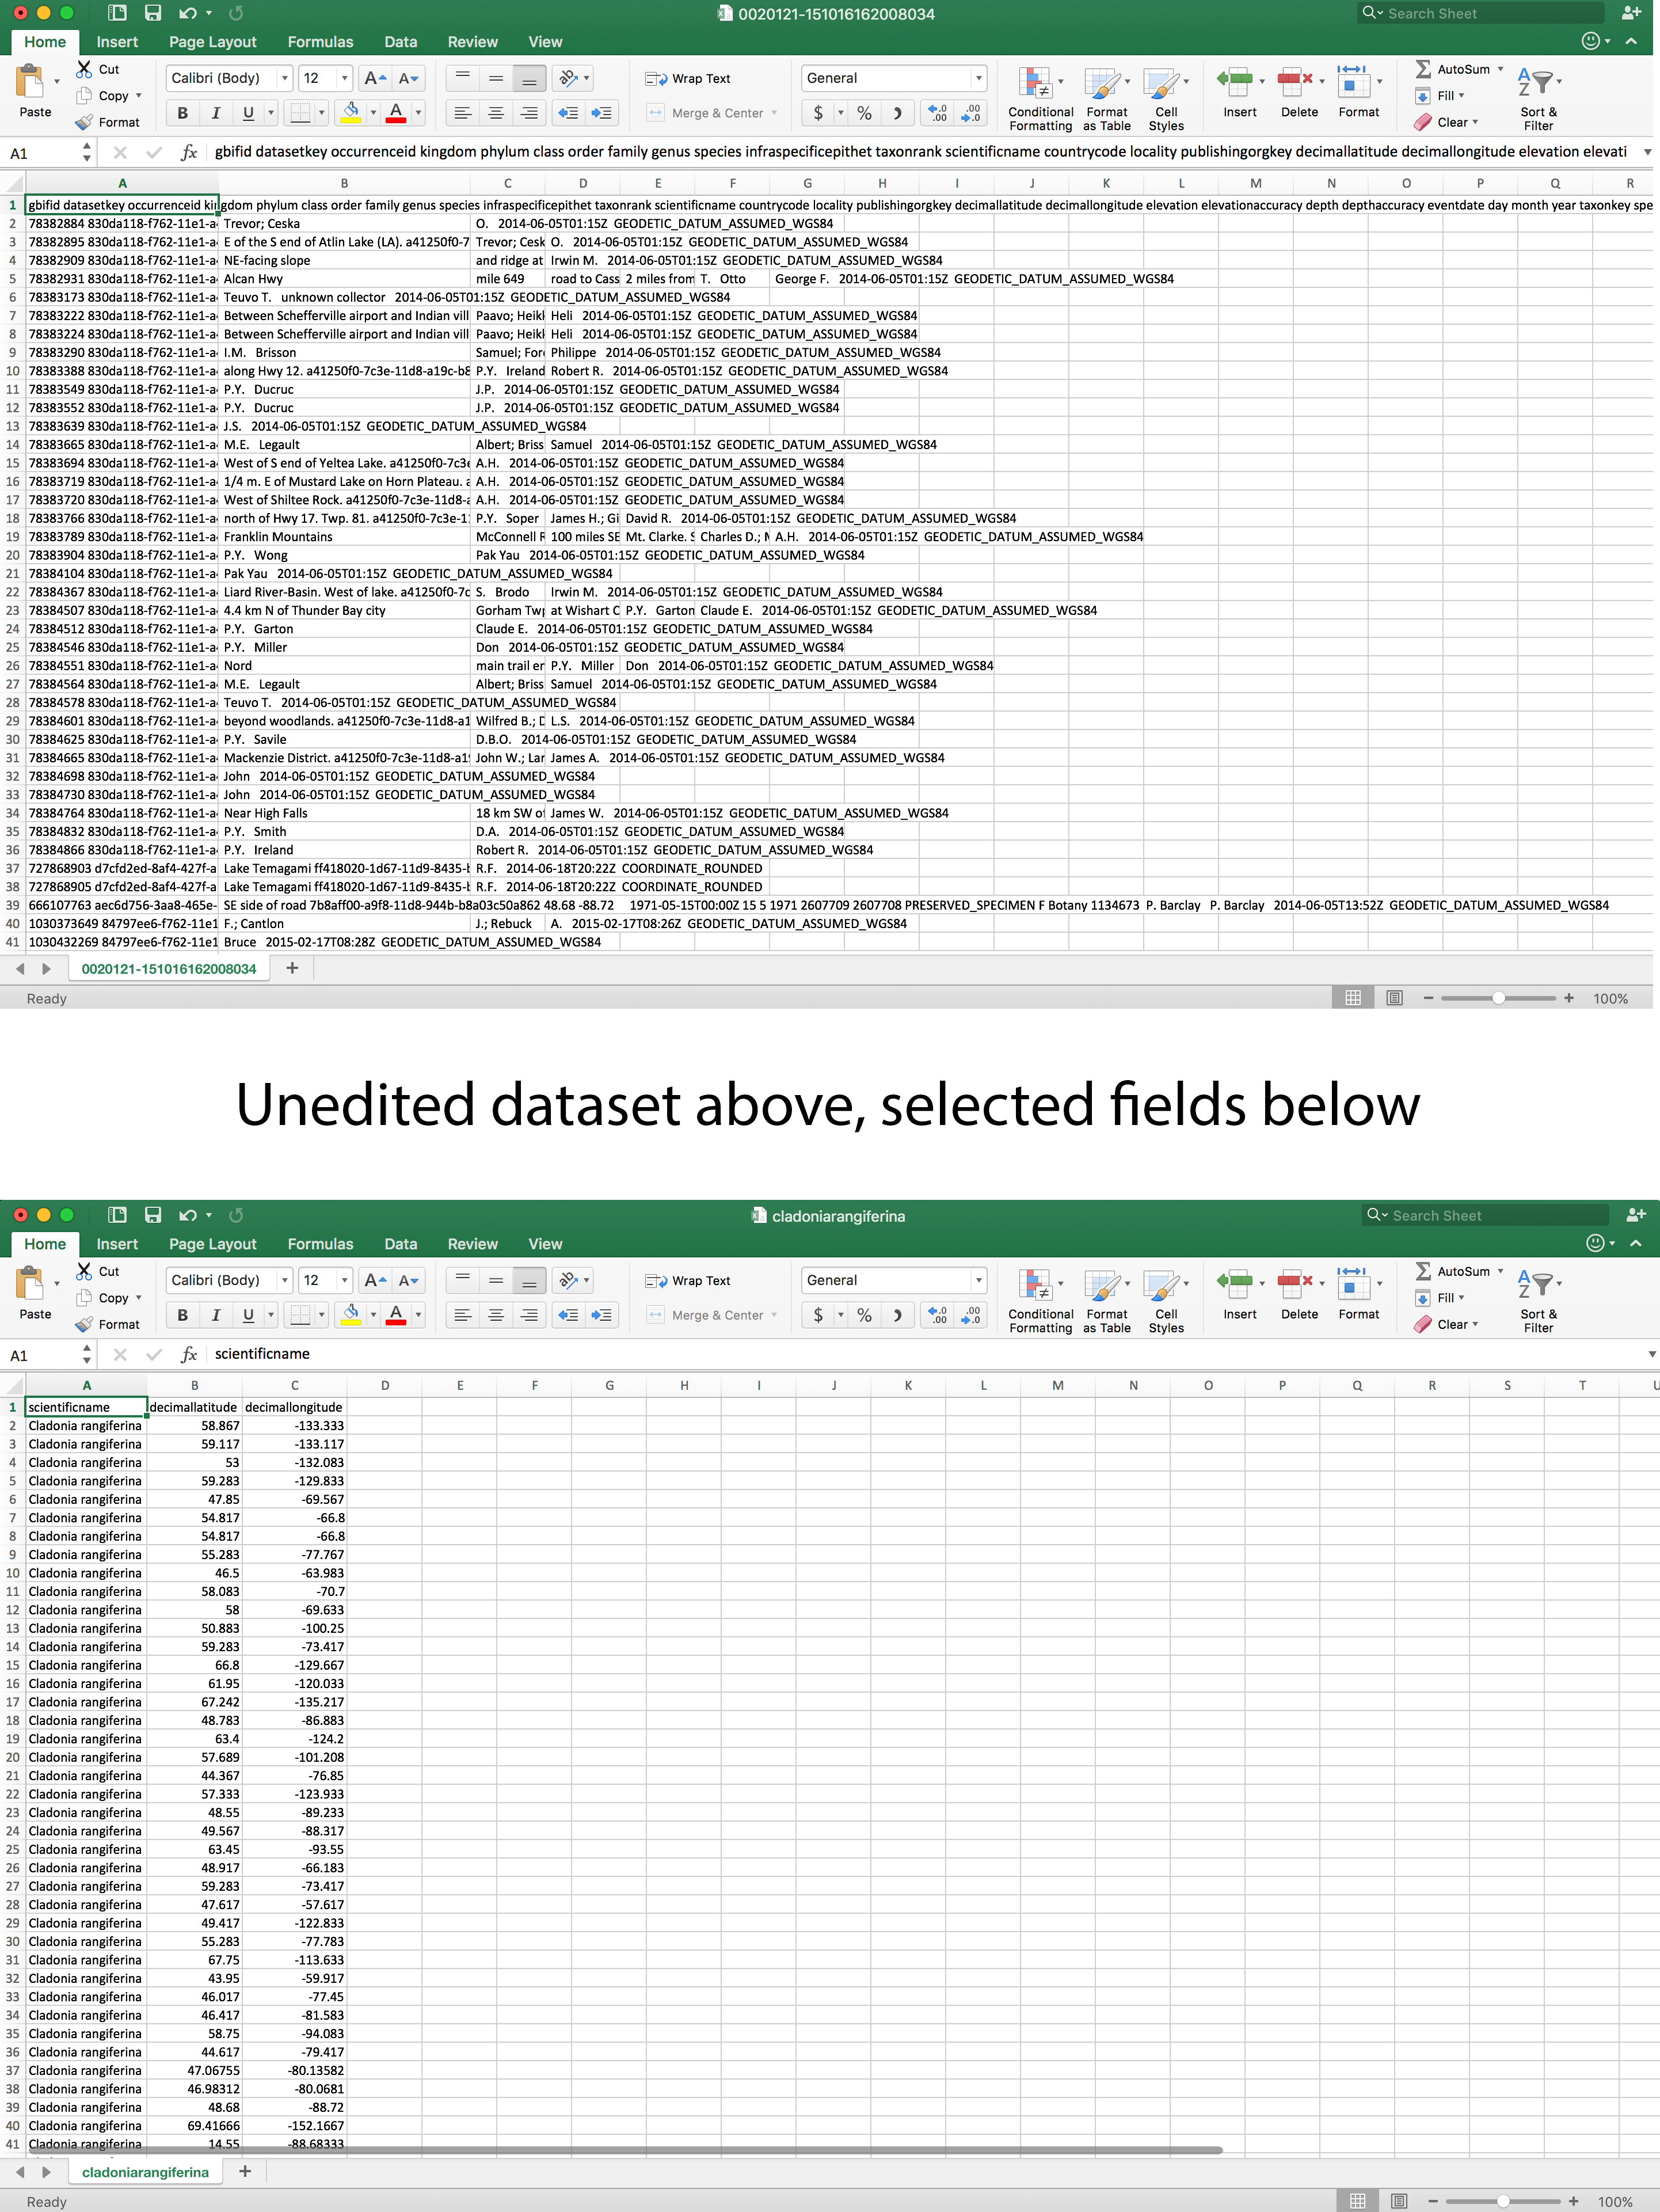
\includegraphics[width=0.7\textwidth]{Figure1}
\caption{Cladonia rangiferina data}
\end{figure}

In order to predict the distribution of each of our three species of interest
in the year 2070, we used maximum entropy modeling (MaxEnt). We used current
global climate data as well as future global climate predictions obtained
from worldclim.org. We decided to use the following four climate variables:
Annual Mean Temperature, Precipitation Seasonality, Precipitation of Driest
Quarter and Precipitation of Warmest Quarter.** These variables should account
for the main differences in climate between now and 2070, and should therefore
have an impact on the possible distributions of all three of our species.
The climate data was downloaded from worldclim.org in raster format, which was
then converted to Ascii (.asc) format using the ArcGIS software. We chose to
download data for 2.5 arc-minute resolution, which gives detailed data for a
small area while keeping the file size manageable. For the future climate data,
we chose to download data from the BCC-CSM1.1 climate model, following the
RCP85 trajectory. The RCP projection simply allows to control for the amount
of greenhouse gas emissions (IPCC). So RCP85 represents one of the more
pessimistic, but realistic, greenhouse gas emission scenarios, where emissions
continue to rise throughout the 21st century, which could happen if nations
do not take policy action to mitigate their emissions. Once all the input data
was correctly obtained and formatted, we ran MaxEnt and obtained the results
in the ‘raw’ format, which is the simplest output format, and just shows the
results of the Maxent model for where the species is more suitable to live in.


\section{Results}
MaxEnt results are shown in the form of maps that indicate the suitability
for where each species is likely to be able to live. Figure 2 shows the
present distribution, and Figure 3 shows the future distribution for
reindeer lichen (Cladonia rangiferina). It is clear that most of the
continent of North America (except for some parts of Mexico) is habitable
for Cladonia rangiferina, and even in 2070, the distribution does not change
too much. \\
\begin{figure}[h!]
\centering
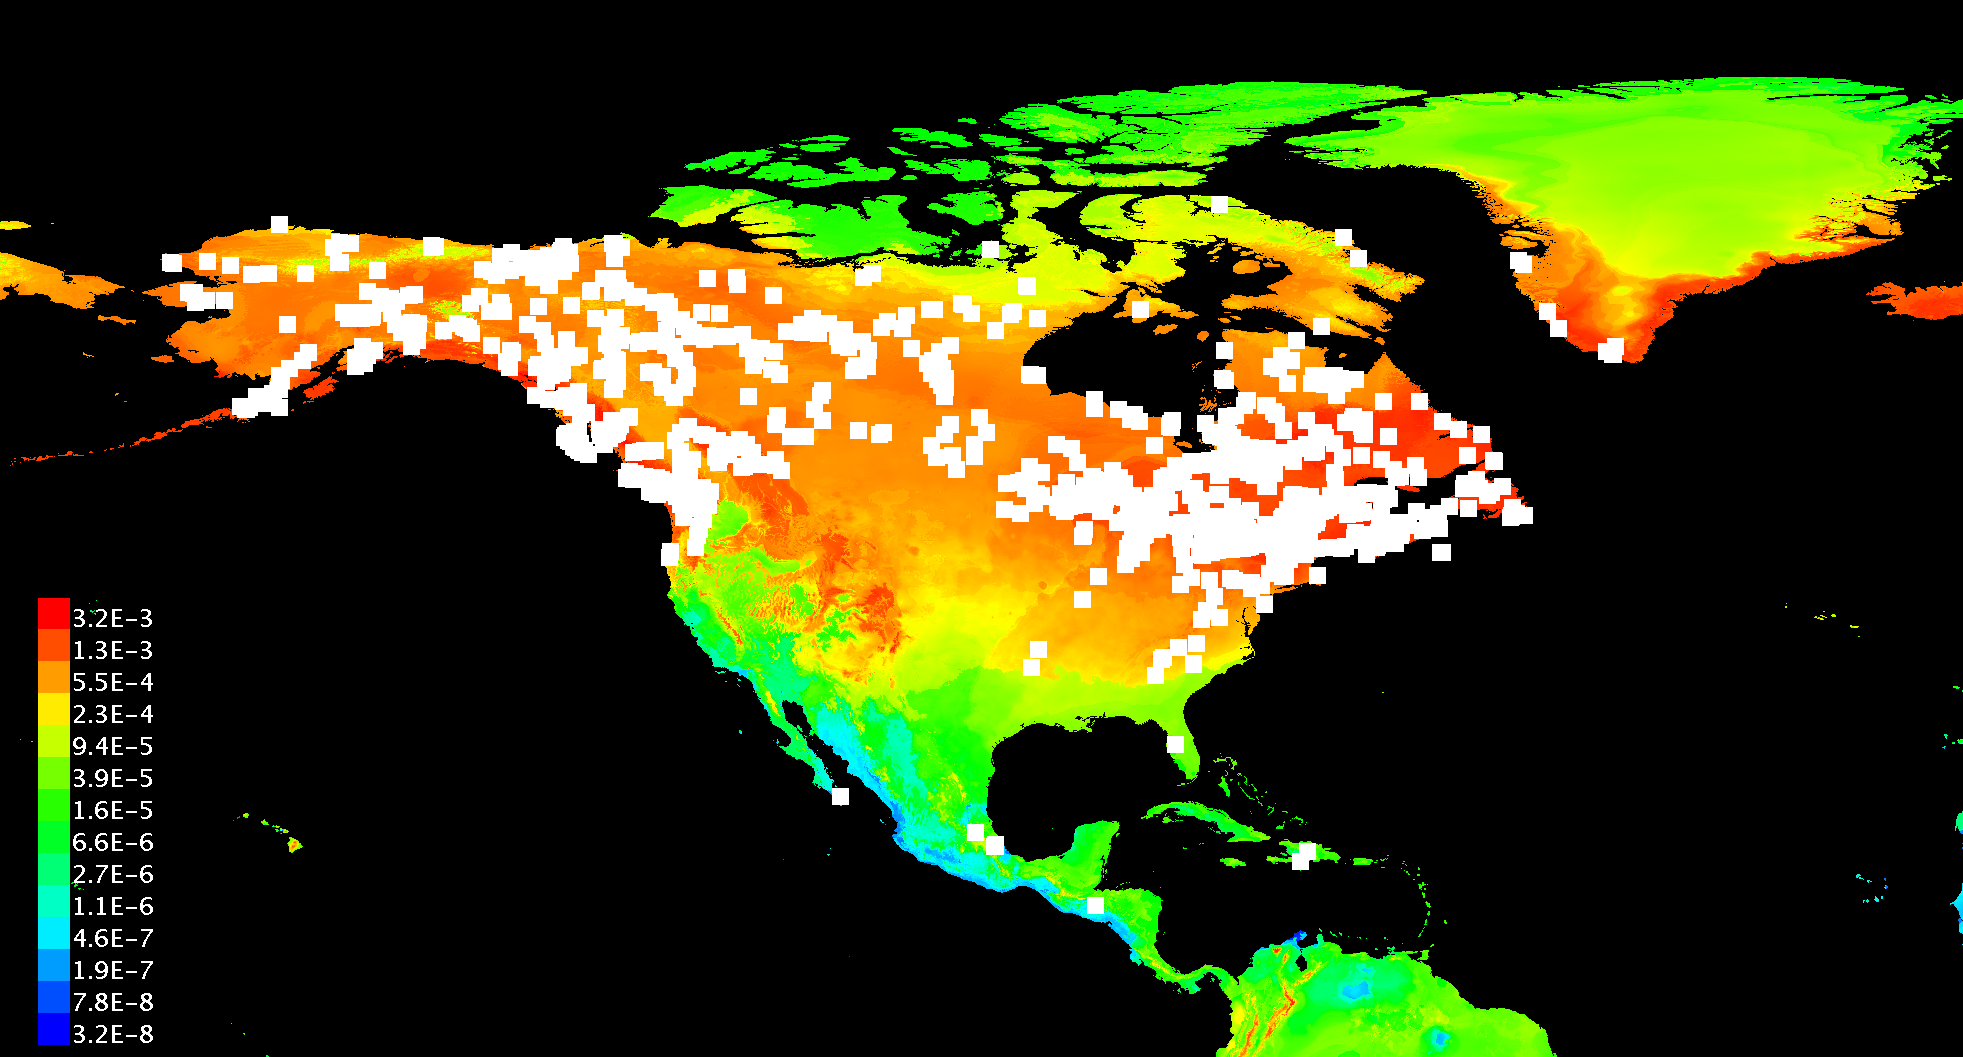
\includegraphics[width=0.7\textwidth]{NCladoniaPresent}
\caption{Distribution of Cladonia Rangiferina in North America}
\end{figure}

\begin{figure}[h!]
\centering
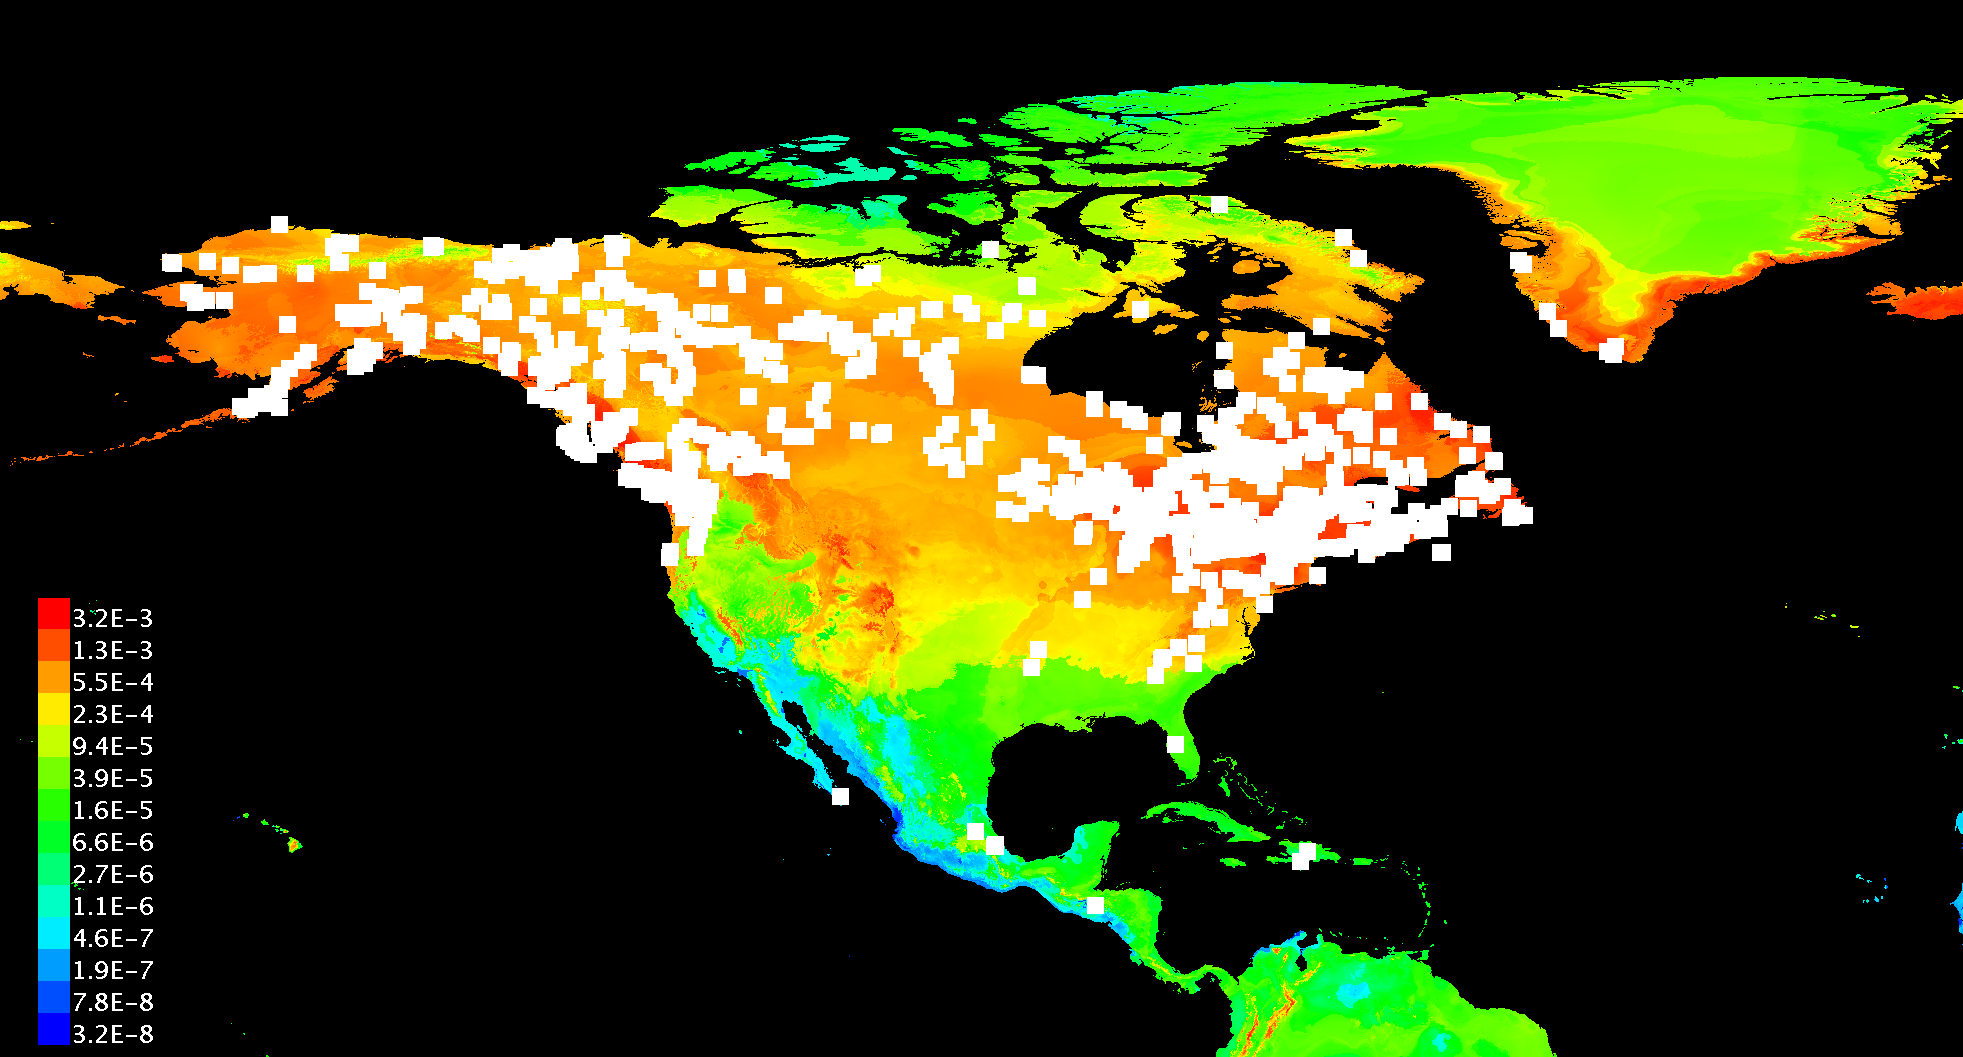
\includegraphics[width=0.7\textwidth]{NCladoniaFuture}
\caption{Distribution of Cladonia Rangiferina in North America}
\end{figure}

Cladonia rangiferina is a very hardy lichen, which can grow in varied conditions
of temperature and precipitation. Unlike many plants, it is also well suited
to very cold climates, which enables it to grow at high latitudes in the
tundra ecosystem. By absorbing moisture directly from the air, it is also able
to thrive in areas with low precipitation. (US Forest Service). This can be
seen in the map because much of Alaska, Northern Canada, and even coastal
Greenland is seen as a suitable habitat for Cladonia rangiferina, whereas
the southern portion of the US is less suitable. By absorbing moisture
directly from the air, it is also able to thrive in areas with low
precipitation. (US Forest Service)\\

Figures 4 and 5 show the current and future distribution of caribou. We
immediately notice that the amount of suitable habitat for caribou noticeably
shrinks between now and 2070, which indicates that climate change will probably
have a significant effect on the current habitat of caribou.

\begin{figure}[h!]
\centering
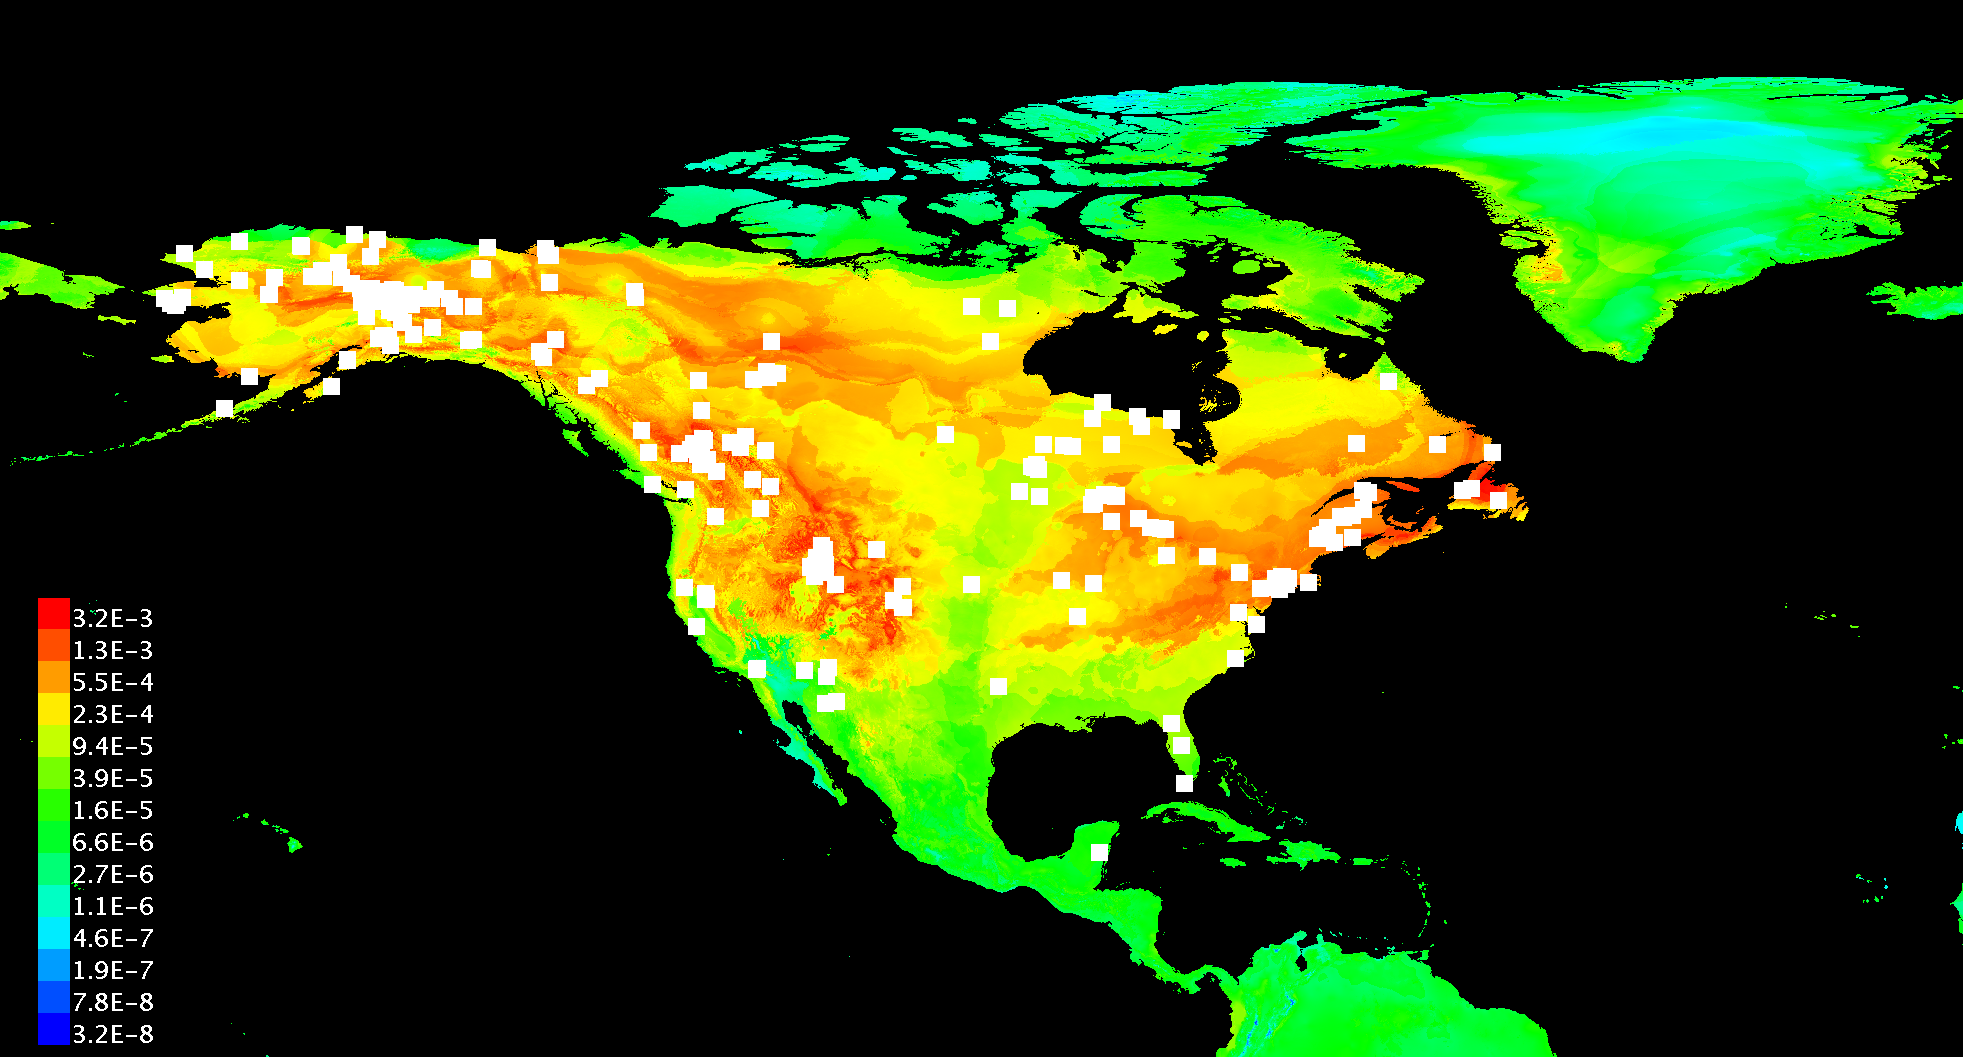
\includegraphics[width=0.7\textwidth]{NCaribouPresent}
\caption{Distribution of Caribou in North America}
\end{figure}

\begin{figure}[h!]
\centering
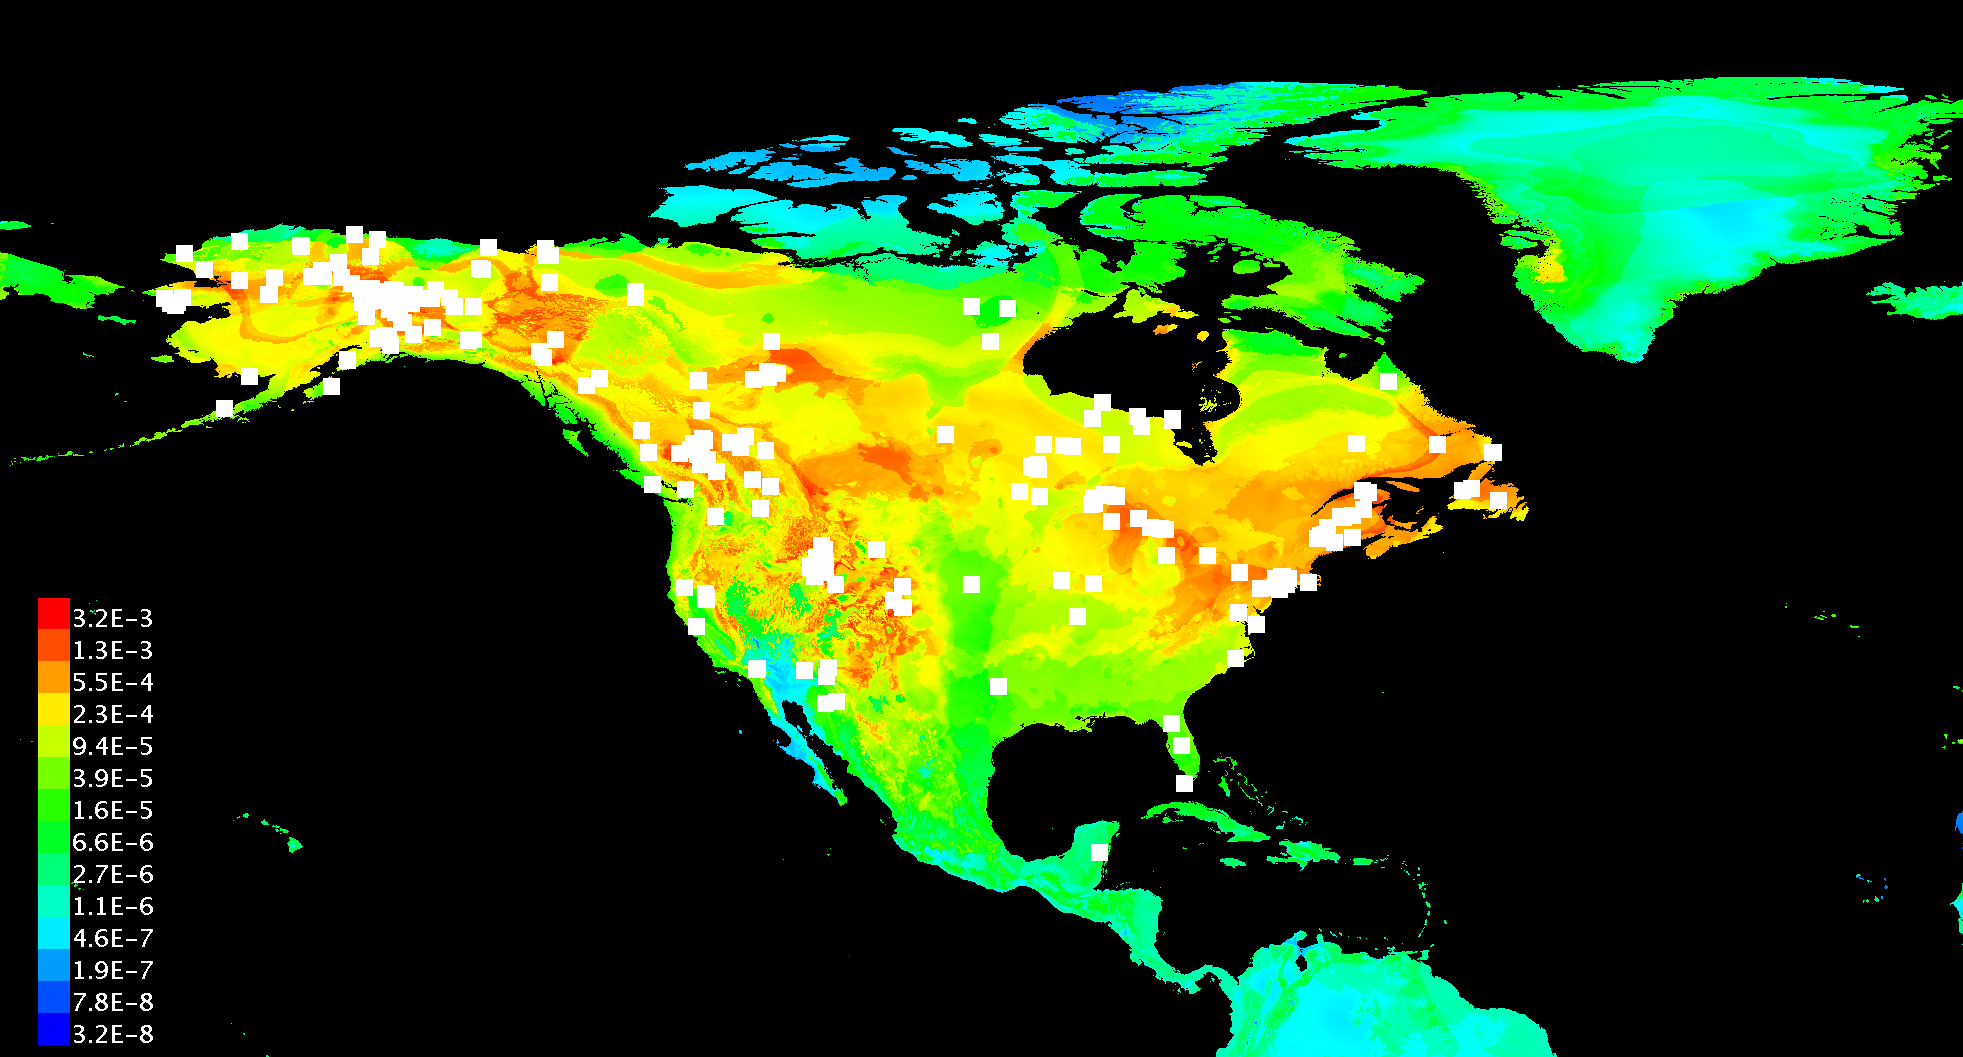
\includegraphics[width=0.7\textwidth]{NCaribouFuture}
\caption{Predicted Caribou habitat for year 2070}
\end{figure}

\section{Discussion}

\small

\bibliographystyle{plain}
\bibliography{final}

\end{document}
